\documentclass[a4paper, 12pt]{report}
\usepackage{amsmath}
\usepackage{amssymb}
\usepackage{graphicx}
\usepackage{float}
\usepackage{tabularx}
\usepackage{booktabs}
\usepackage[page, toc]{appendix}
\usepackage{hyperref}

\hypersetup{
	colorlinks=true,
	linkcolor=black
}

\begin{document}
	\pagenumbering{gobble}
	\begin{titlepage}
		\makebox[\textwidth]{\large  Department of Electrical and Electronic Engineering}
		\vspace*{1.5cm}
		\makebox[\textwidth]{\large University of Johannesburg}
		\makebox[\textwidth]{\textbf{EEP3B21 2018}}
		\vspace*{1.5cm}
		\makebox[\textwidth]{\textit{Lecturer: Dr. AR Ndjiongue}}
		\makebox[\textwidth][l]{\large SIGNALS}
		\vspace*{1.5cm}
		\makebox[\textwidth][r]{\large Group Project}
		\vspace*{0.5cm}
		\makebox[\textwidth]{\LARGE Practical Project Report 1}
		\vspace*{0.1cm}
		\makebox[\textwidth]{\large Ruan de Bruyn - 216054484}
		\vspace*{0.1cm}
		\makebox[\textwidth]{\large Quintin Kruger - 216054484}
		\vspace*{0.1cm}
		\makebox[\textwidth]{\large Wesley Richardson - 216054484}
		\makebox[\textwidth]{\today}
		\vfill
		\noindent I hereby declare that, except where specifically indicated, the work submitted herein is my own original work\\
		Signed: \hspace*{5cm} Date:
	\end{titlepage}

	\pagenumbering{roman}
	\tableofcontents
	\newpage
	\pagenumbering{arabic}

	\chapter{Discrete-Time Signals and Systems} % (fold)
	\label{cha:discrete_time_signals_and_systems}
		\section{Sampling and Aliasing} % (fold)
		\label{sec:sampling_and_aliasing}
			The first part of this practical is conducted with the purpose of simulating digital sampling of analog signals with Octave, and identifying the aliasing artifact that appears when signals are not sampled adequately. The aliasing artifact is closely tied to the Sampling Theorem, which states that a band-limited signal, having no frequency components above $f_h$ Hz, is completely specified by samples that are taken at a uniform rate greater than $2f_h$ Hz; that is, if the time between samples is no greater than $\frac{1}{2f_h}$ seconds.

			With that in mind, we simulate the digital sampling of an analog signal with the equation
			\begin{equation}
				x(t,f) = \sin(2\pi f t)
				\label{eq:analog}
			\end{equation}
			\noindent with the following code in Octave:\par
			\texttt{t = linspace(0,1,101);}\par
			\texttt{f=1; s=sin(2*pi*f*t);}\par

			\vspace*{1em}\noindent Since the time array consists of 100 samples in the time interval of one second, our sampling frequency is $f_s = 100 \text{Hz}$, with sampling period $T_s = 1/100$, and the variable \texttt{f} stores the frequency of the sine wave. This renders equation \ref{eq:analog} into a digital form represented by
			\begin{equation}
				\begin{array}{rcl}
					x(n, f) & = & \sin(2\pi fnT_s) \\
					& = & \sin\left(\frac{2\pi f n}{100}\right)\\
					& = & \sin\left(\frac{\pi}{50}fn\right), \quad n \in \mathbb{Z}
				\end{array}
				\label{eq:digital}
			\end{equation}

			Plotting \ref{eq:digital} with $f=1$ Hz, we have
			\begin{figure}[H]
				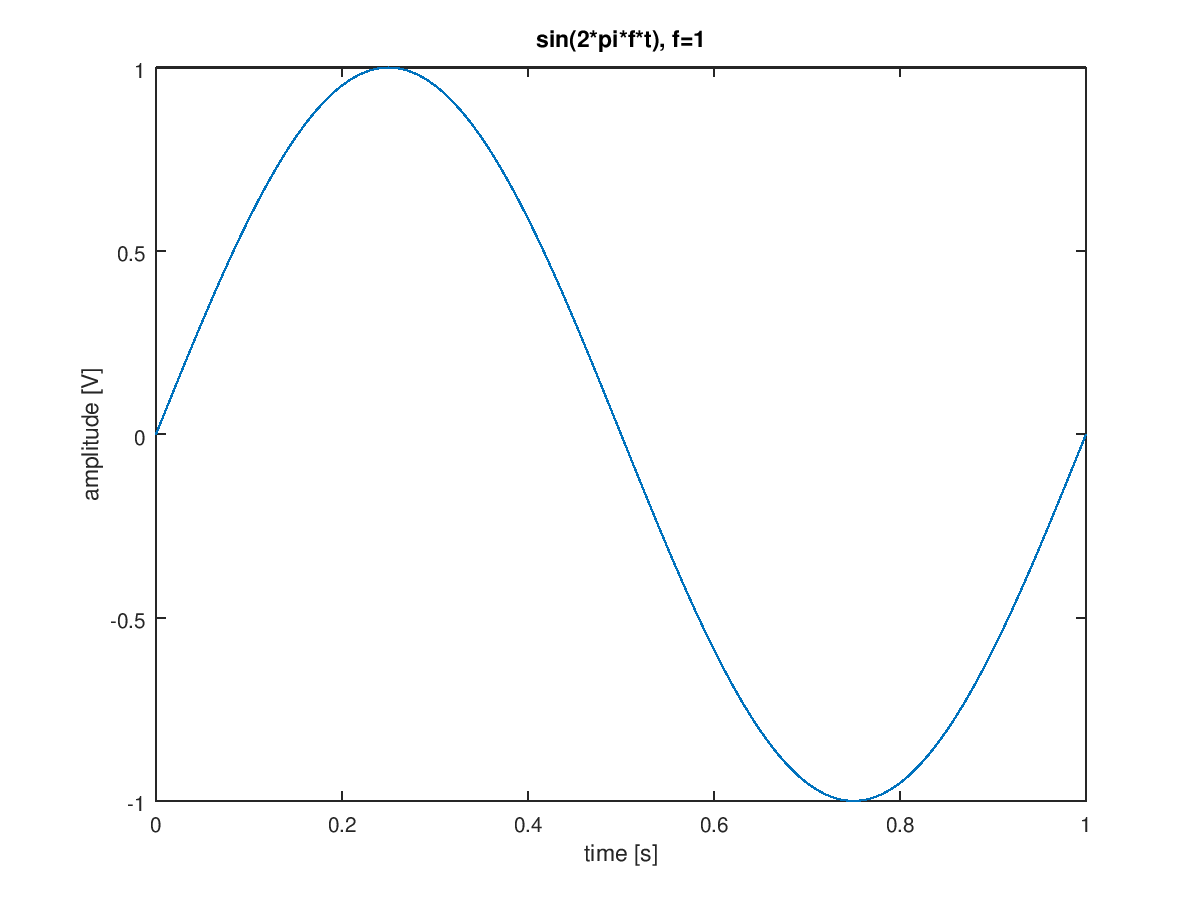
\includegraphics[width=\textwidth]{img/1_1.png}
				\caption{$x(n, 1)$}
				\label{fig:1}
			\end{figure}

			Closely inspecting figure \ref{fig:1}, it is exactly what we expect it to be, and looks identical to a continuous sine wave, with no visible effects from discrete samples. We will inspect more samples in the following figures.

			\begin{figure}[H]
				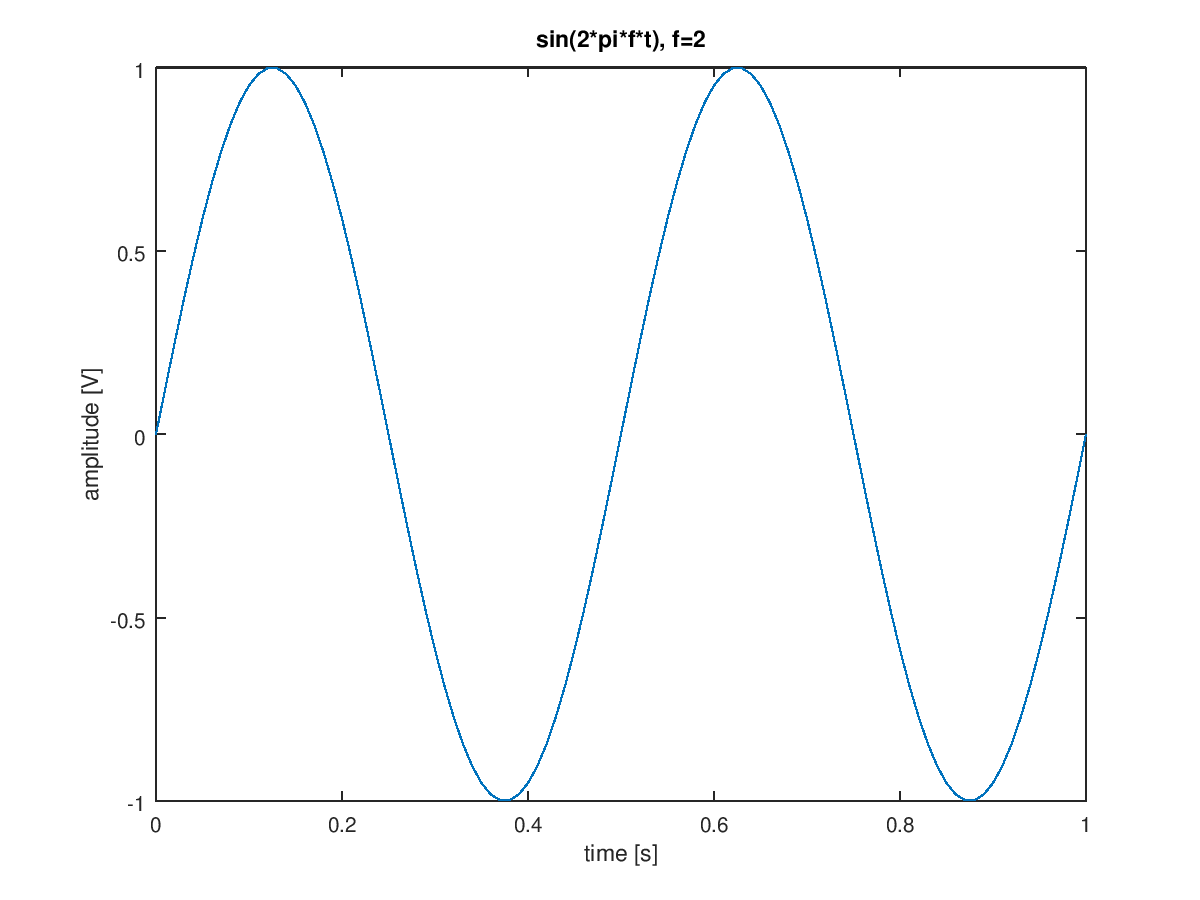
\includegraphics[width=\textwidth]{img/1_2.png}
				\caption{$x(n, 2)$}
				\label{fig:2}
			\end{figure}

			\begin{figure}[H]
				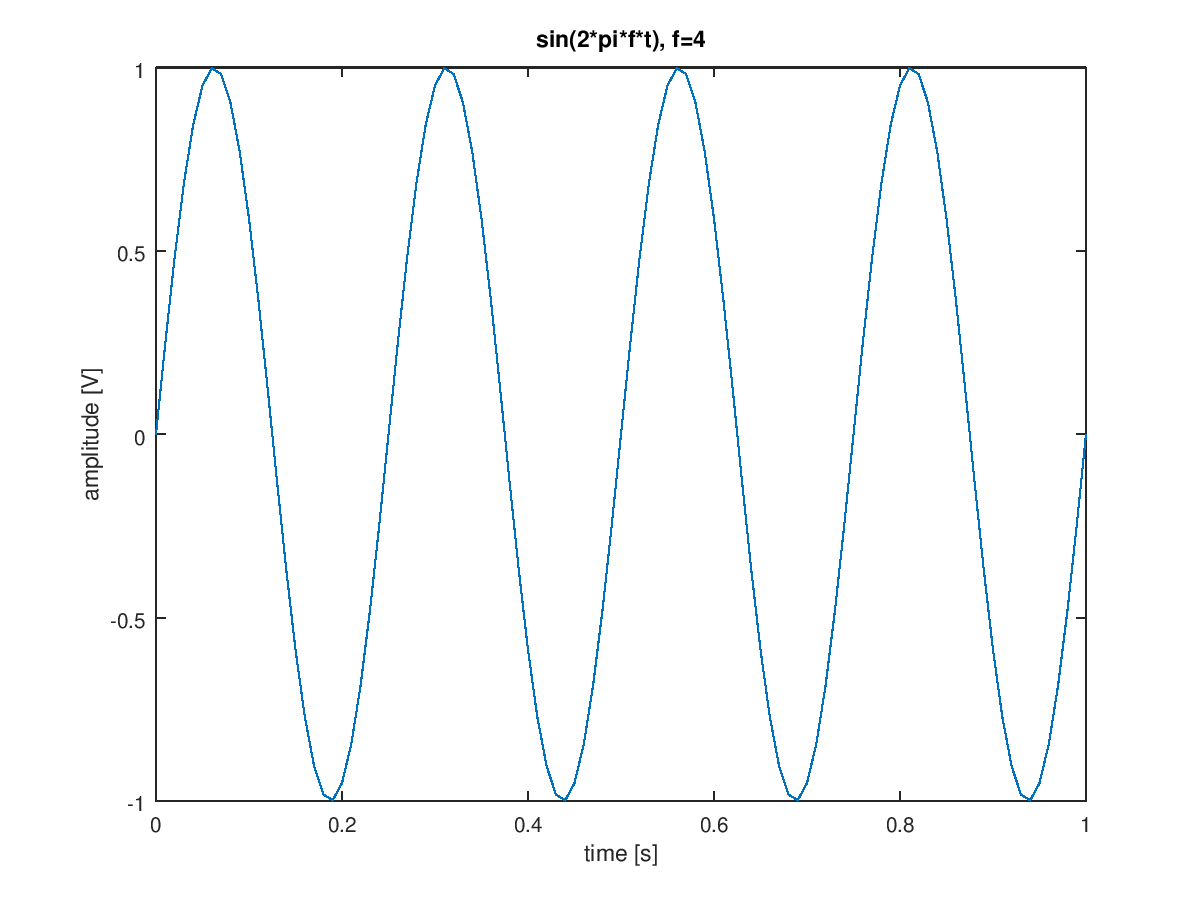
\includegraphics[width=\textwidth]{img/1_3.png}
				\caption{$x(n, 4)$}
				\label{fig:3}
			\end{figure}

			In figure \ref{fig:3}, when $f=4$ Hz, we can start seeing the first signs of sampling artifacts toward the peaks of the sine wave. However, it is still easily verifiable by inspection that the signal is in fact a sine wave which has 4 periods in the span of a second, thereby having a frequency of 4 Hz.

			\begin{figure}[H]
				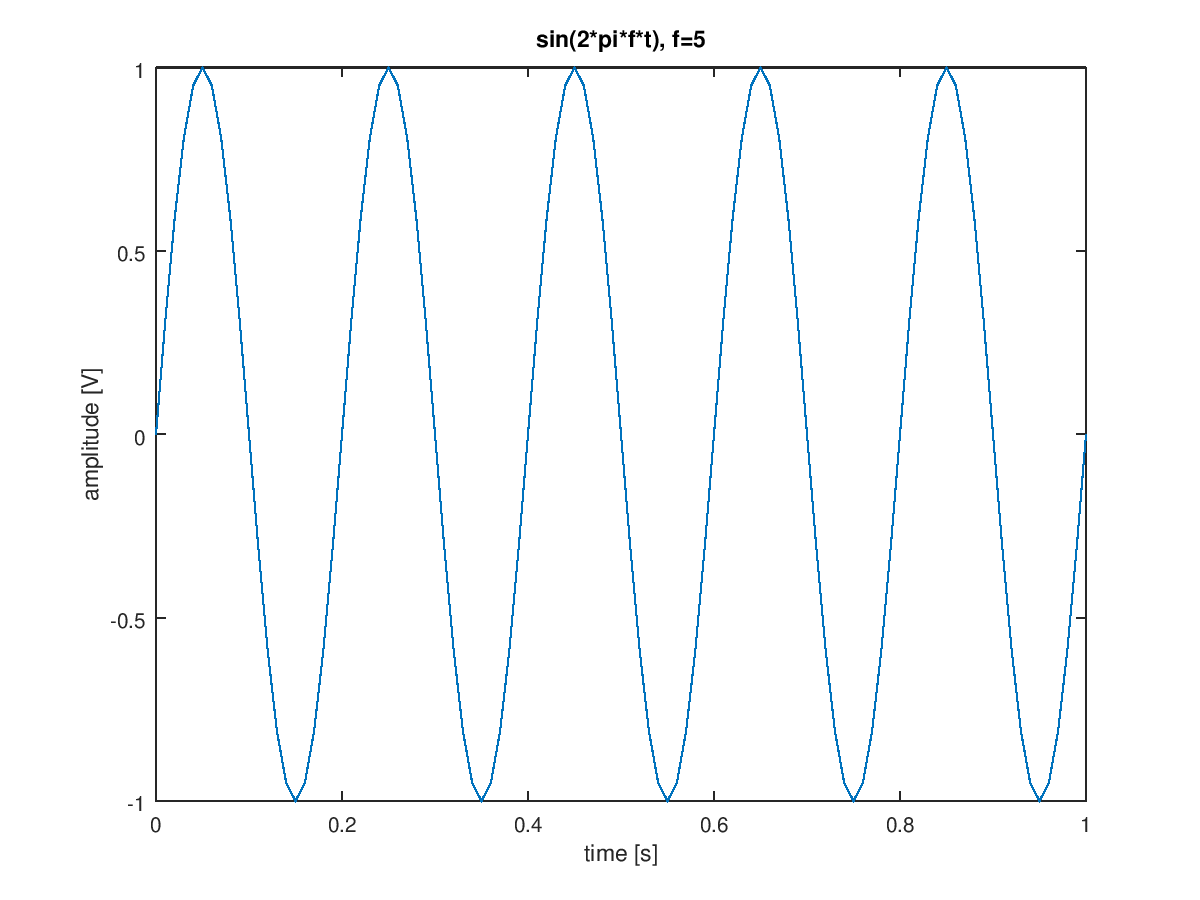
\includegraphics[width=\textwidth]{img/1_4.png}
				\caption{$x(n, 5)$}
				\label{fig:4}
			\end{figure}

			\begin{figure}[H]
				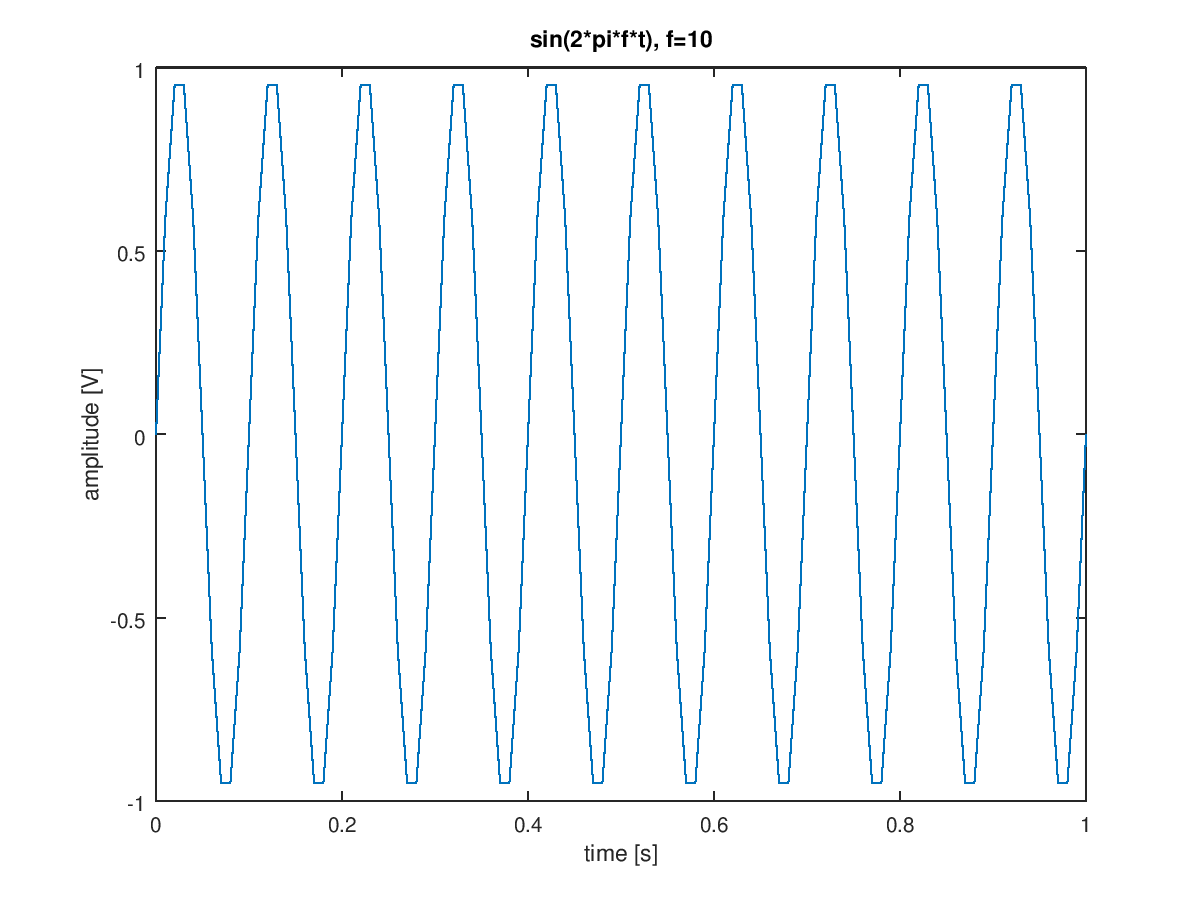
\includegraphics[width=\textwidth]{img/1_5.png}
				\caption{$x(n, 10)$}
				\label{fig:5}
			\end{figure}

			In figure \ref{fig:5} we can start seeing a more pronounced sampling effect, as the sampling period now misses the peaks of the sine wave entirely.

			\begin{figure}[H]
				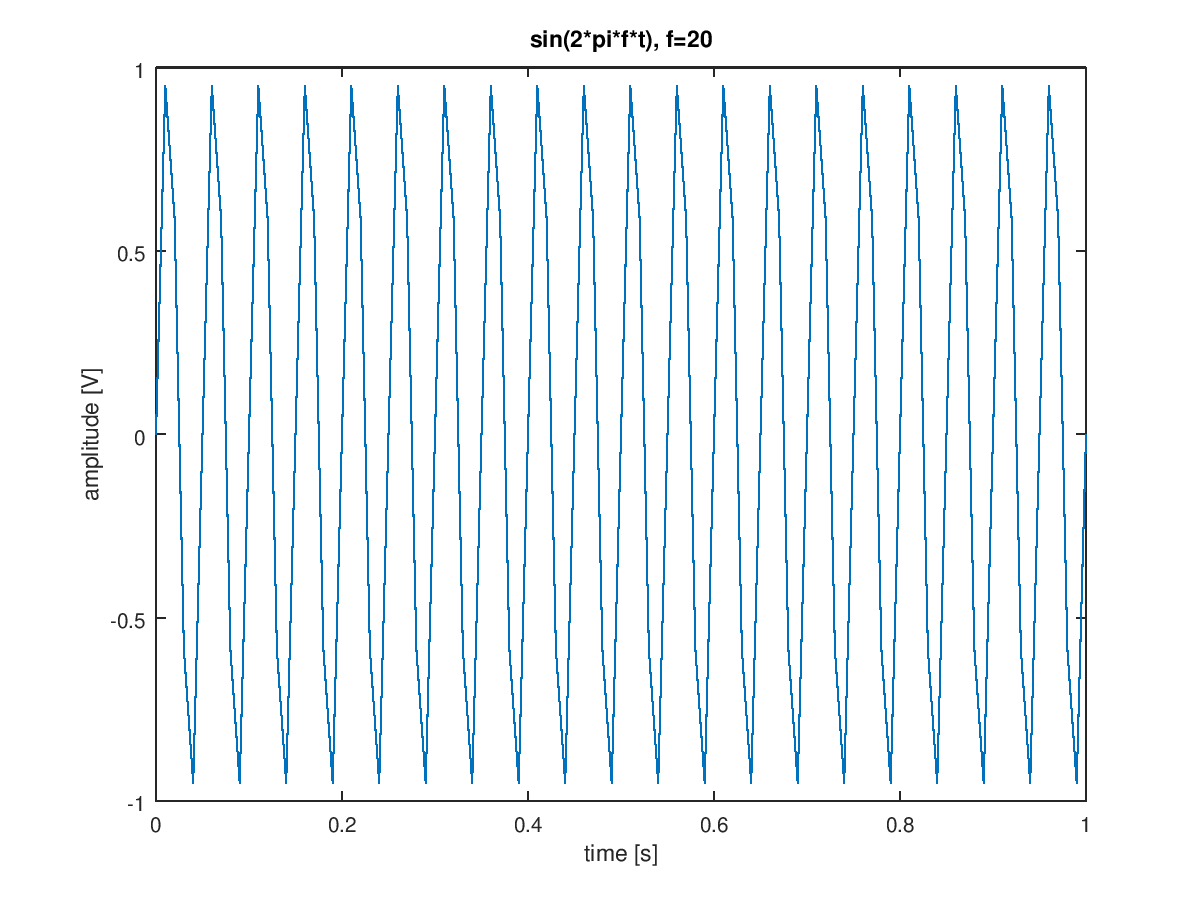
\includegraphics[width=\textwidth]{img/1_6.png}
				\caption{$x(n, 20)$}
				\label{fig:6}
			\end{figure}

			\begin{figure}[H]
				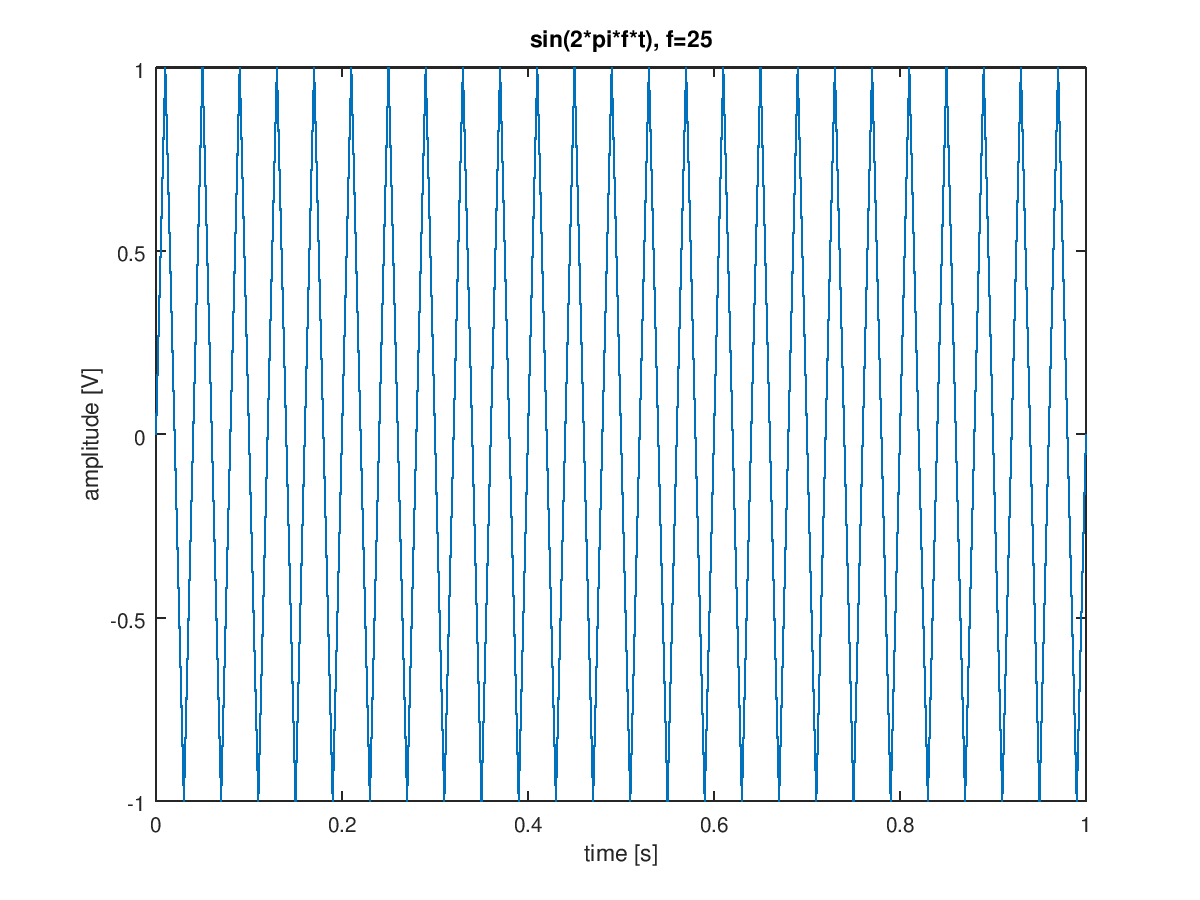
\includegraphics[width=\textwidth]{img/1_7.png}
				\caption{$x(n, 25)$}
				\label{fig:7}
			\end{figure}

			\begin{figure}[H]
				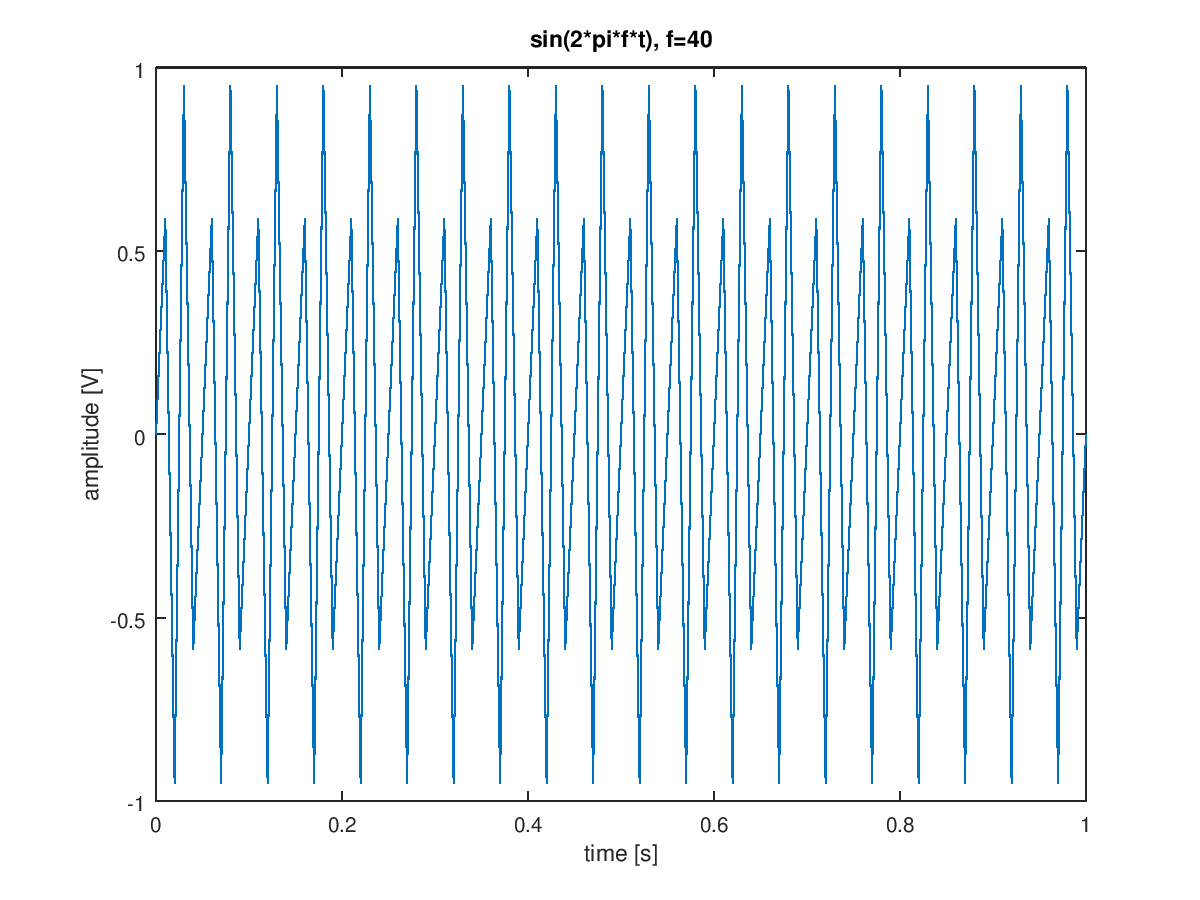
\includegraphics[width=\textwidth]{img/1_8.png}
				\caption{$x(n, 40)$}
				\label{fig:8}
			\end{figure}

			Looking at figure \ref{fig:8}, it is no longer possible to visually identify the sample being a sine wave, although one may allude so from its clear and consistent periodicity. This is at $f=40$ Hz, fast approaching the Nyquist frequency $f_n = 50$ Hz.

			\begin{figure}[H]
				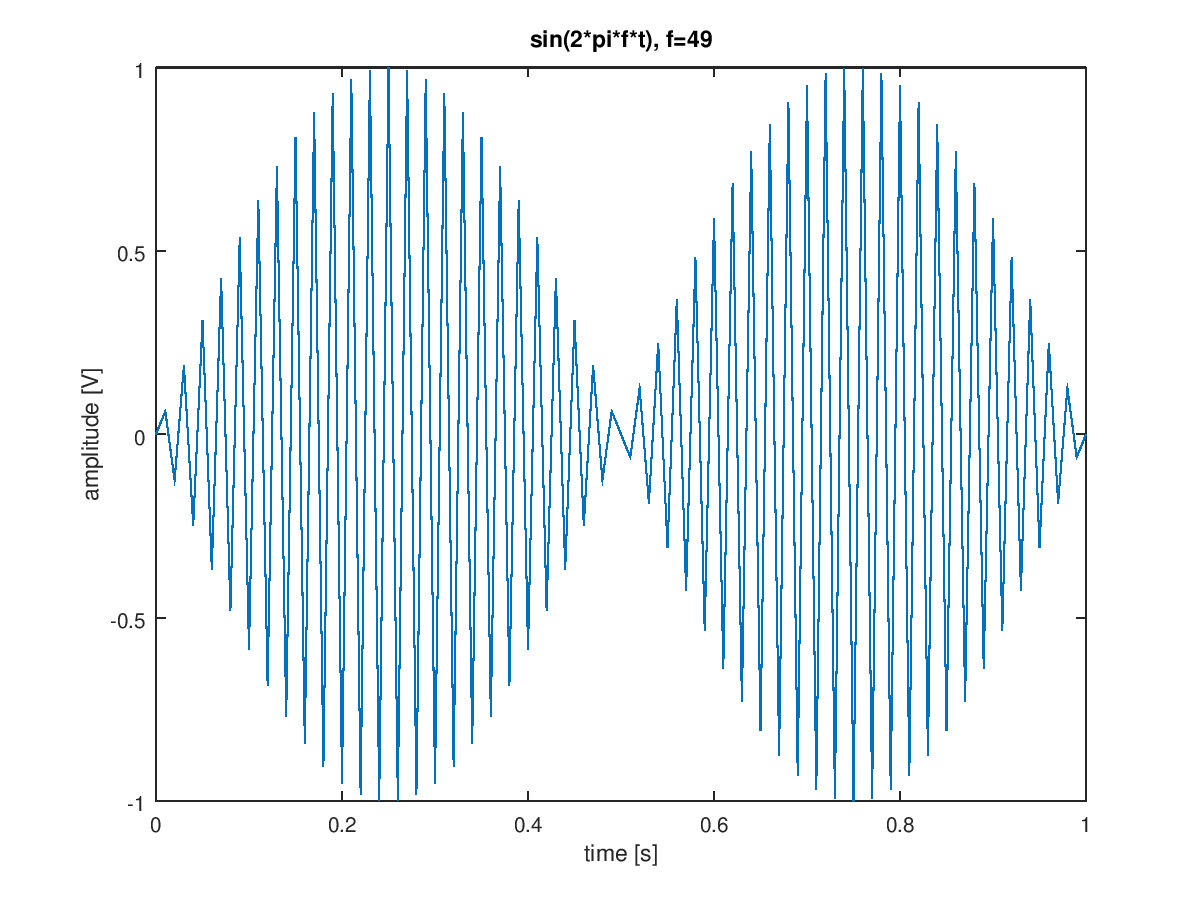
\includegraphics[width=\textwidth]{img/1_9.png}
				\caption{$x(n, 49)$}
				\label{fig:9}
			\end{figure}

			\begin{figure}[H]
				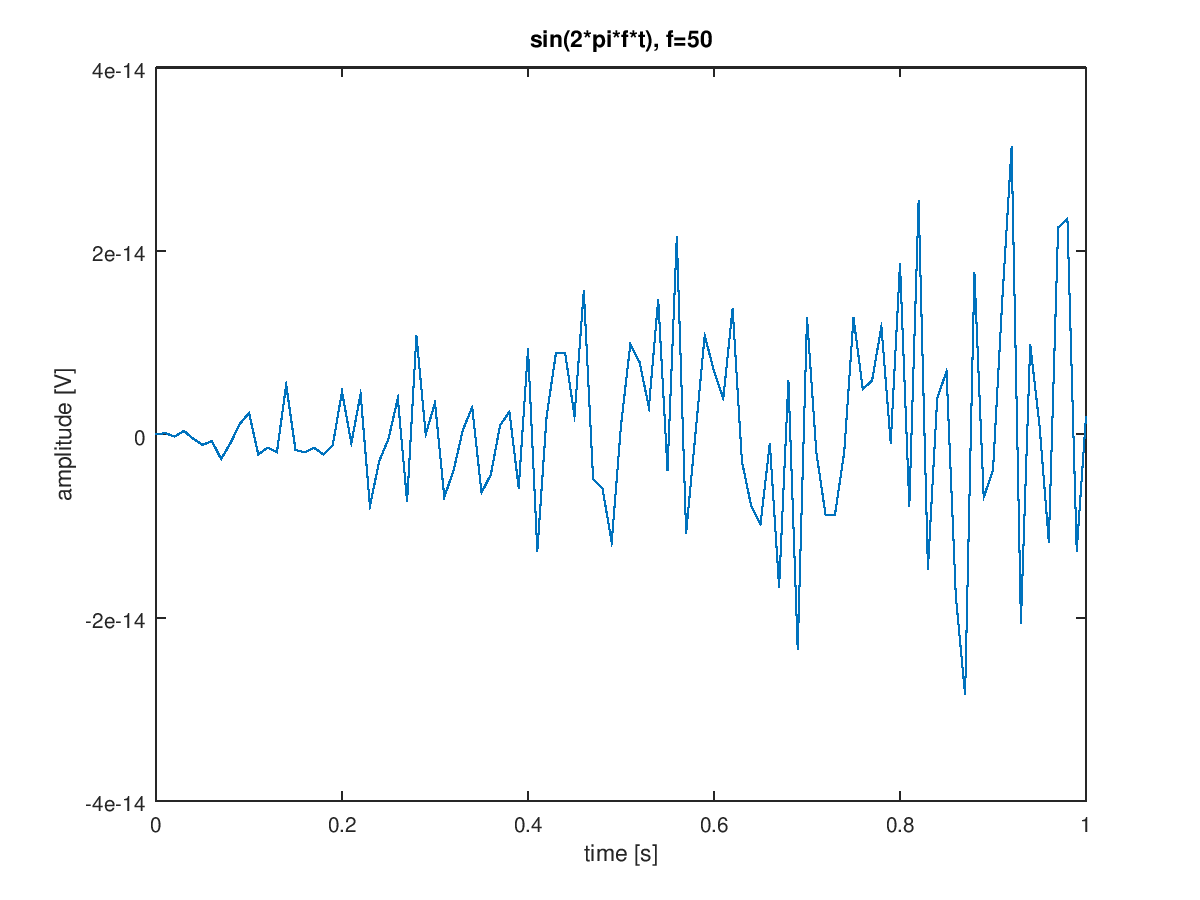
\includegraphics[width=\textwidth]{img/1_10.png}
				\caption{$x(n, 50)$}
				\label{fig:10}
			\end{figure}

			In figure \ref{fig:9} there are significant deviations from the original signal. In figure \ref{fig:10}, the resulting signal is completely unrecognizable. Unlike all of the previous figures, figure \ref{fig:10} bears no resemblance to a sine wave, and does not even appear to be periodic. Its amplitude is also much smaller, as can easily be seen. While the sine wave we are sampling has a maximum amplitude of 1, by inspection we estimate that the signal in this figure has a maximum amplitude of $3\times10^{-14}$, which is incredibly small. One might wonder where the rest of the signal has been lost, as we do receive those peaks as input. Slightly shifting the signal by $1/200$ of a second, we sample the peaks of the input signal once more, as seen in figure \ref{fig:11}.

			\begin{figure}[H]
				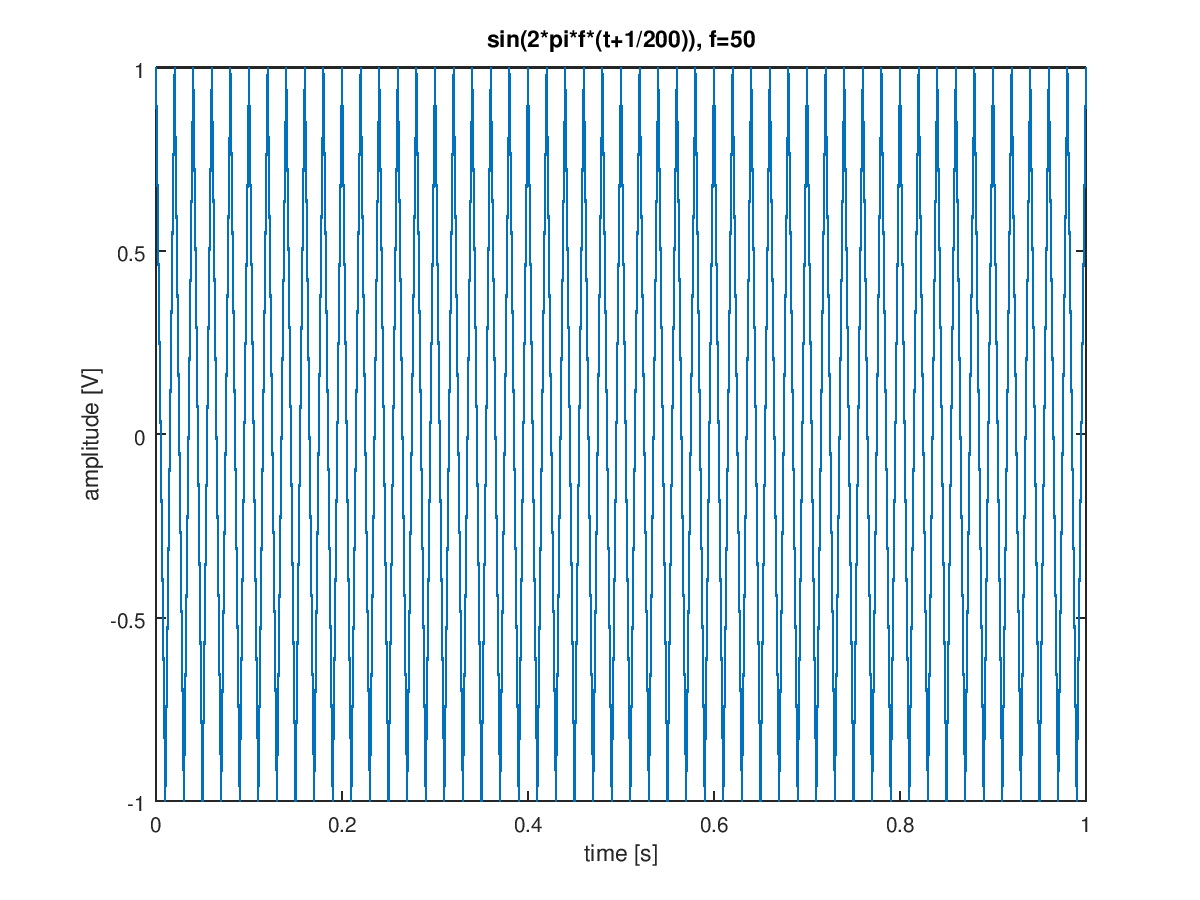
\includegraphics[width=\textwidth]{img/1_11_shift.png}
				\caption{Time-shifted sine wave}
				\label{fig:11}
			\end{figure}

			In order to see further explore the phenomena we have seen so far, we inspect the sampled frequencies for $\pm f, f \in \{25, 75\}$. The results for $f = -25$ Hz is given in \ref{fig:12}. Predictably, since $f < f_n$, the signal is sampled adequately. Notice that we have already sampled $f = 25$ Hz in \ref{fig:7}, and the two signals look almost identical, except for a phase shift of $\pi$ rad. To illustrate the difference between the function, we look to \ref{fig:13} and \ref{fig:14}, whose respective peak amplitudes imply that the signals reinforce each other, despite being $\pi$ radians out of phase. However, this is if the numerical difference between them is taken. Adding them, then, should intuitively have the opposite effect, and have them cancel out. Figure \ref{fig:15} confirms this intuition, and the signals cancel out.

			\begin{figure}[H]
				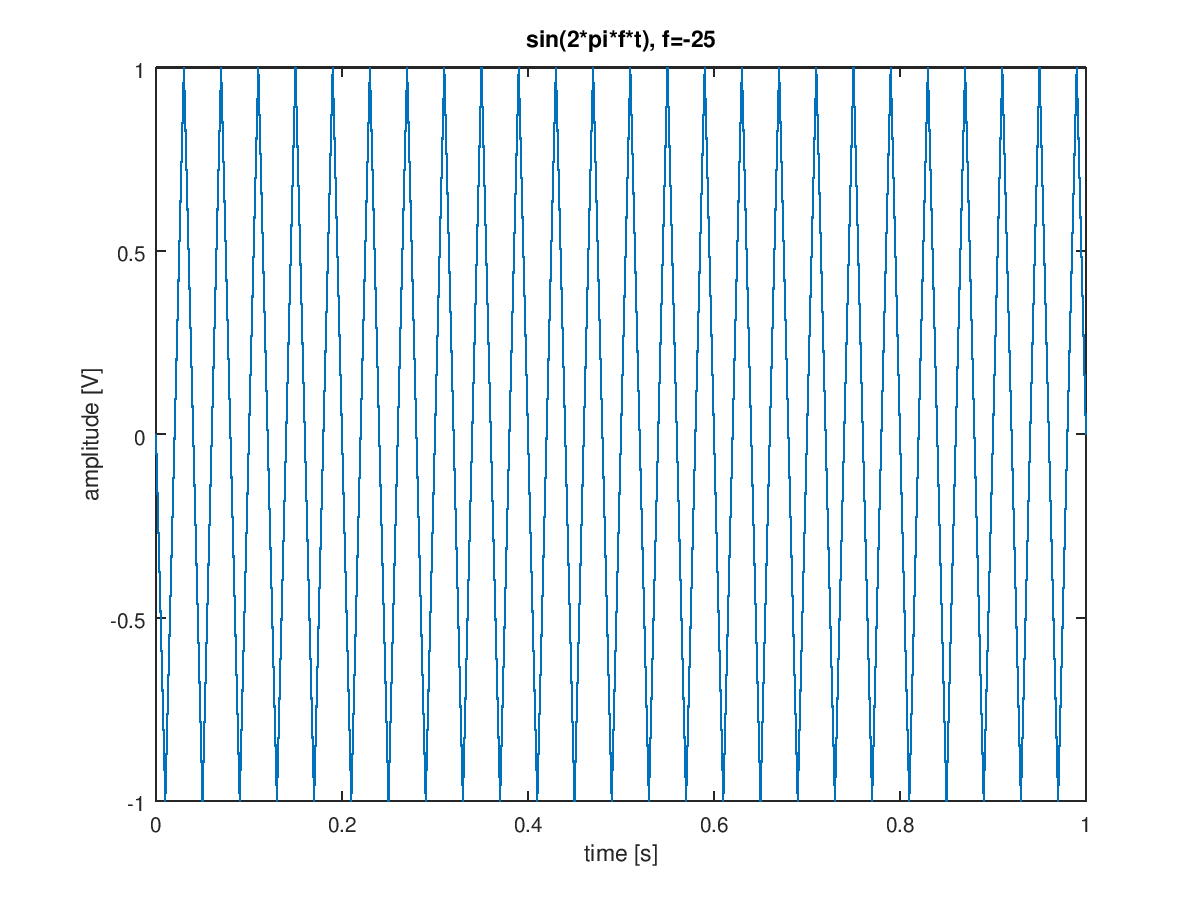
\includegraphics[width=\textwidth]{img/1_12_-25.png}
				\caption{$x(n, -25)$}
				\label{fig:12}
			\end{figure}

			\begin{figure}[H]
				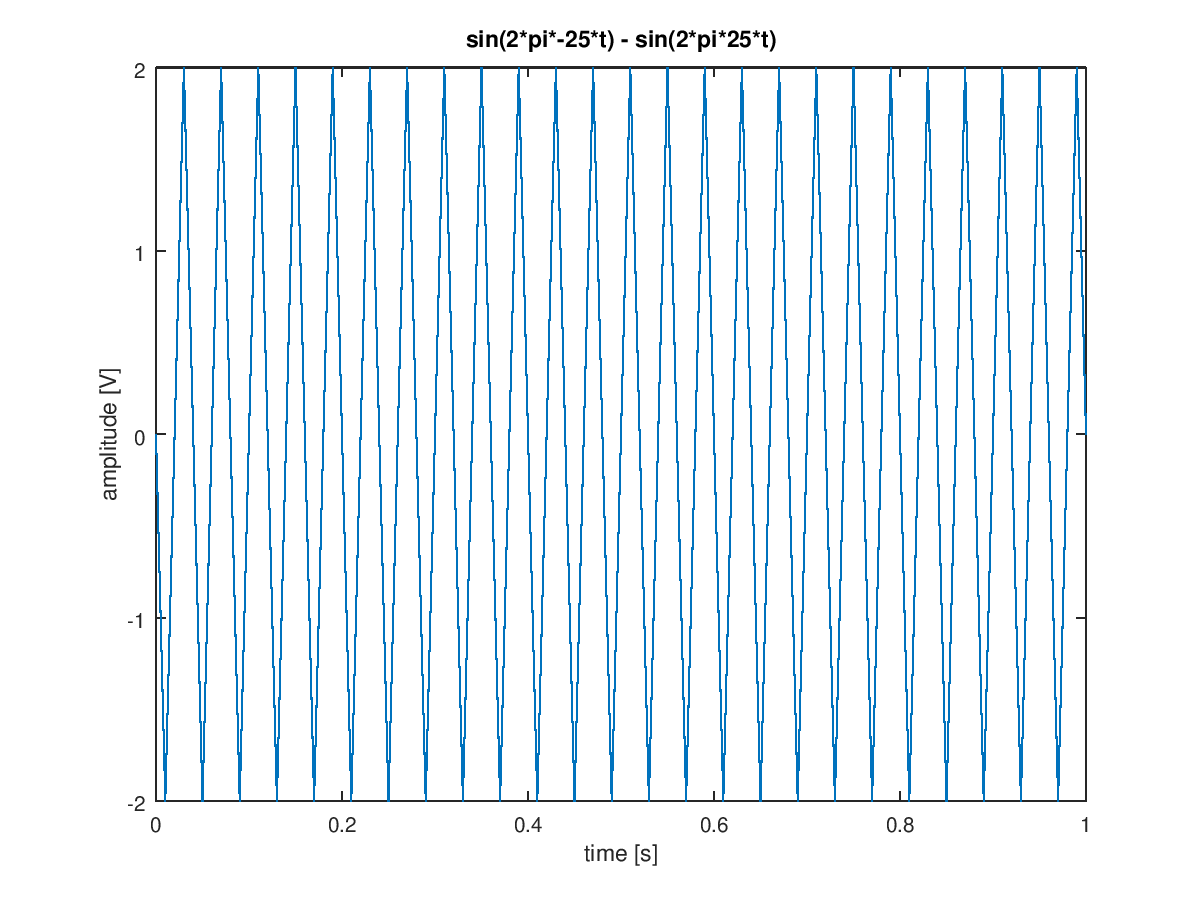
\includegraphics[width=\textwidth]{img/1_13_diff.png}
				\caption{$x(n, -25) - x(n, 25)$}
				\label{fig:13}
			\end{figure}

			\begin{figure}[H]
				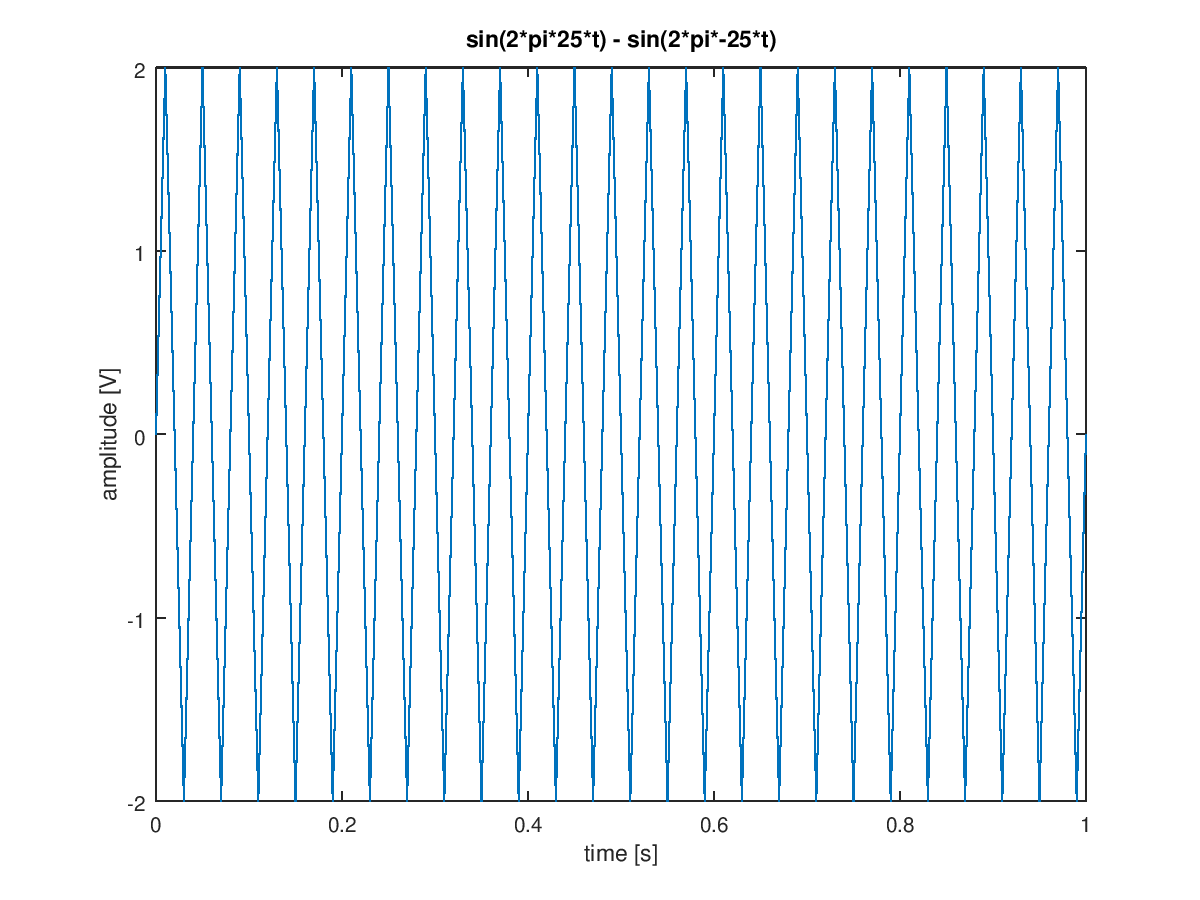
\includegraphics[width=\textwidth]{img/1_14_diff.png}
				\caption{$x(n, 25) - x(n, -25)$}
				\label{fig:14}
			\end{figure}

			\begin{figure}[H]
				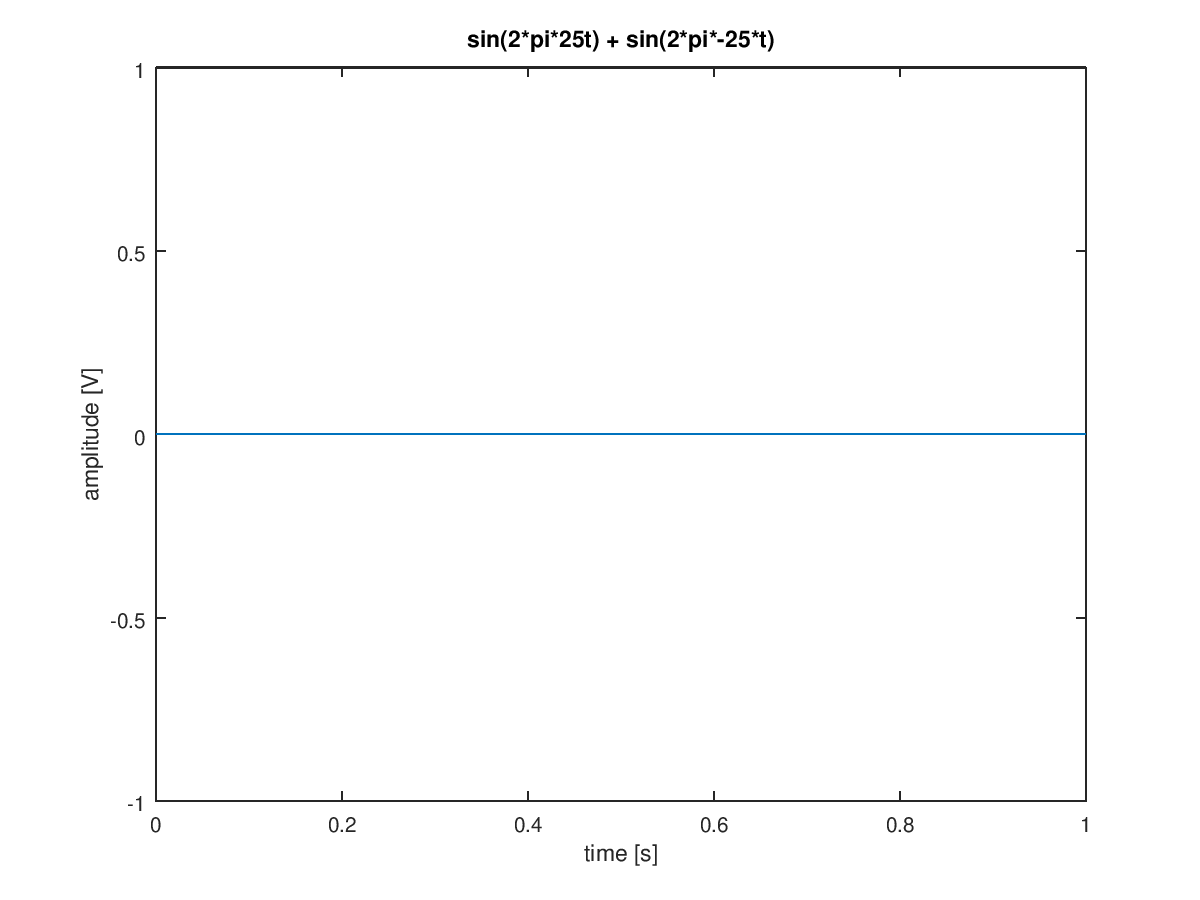
\includegraphics[width=\textwidth]{img/1_15_cancel.png}
				\caption{$x(n, 25) + x(n, -25)$}
				\label{fig:15}
			\end{figure}

			For the sake of brevity, we have avoided adding the results for repeating all of the above experiments with a cosine function, as the results are the same, except all signals are shifted $\pi/2$ radians to the right. However, what if we repeat them using $f=\pm75$ Hz, where $|f| > f_n$? If we compare figure \ref{fig:12} and \ref{fig:16}, something truly interesting arises. Both signals appear to be the exact same. Even though $f=75$ Hz should oscillate three times as fast as $f=-25$ Hz, these oscillations are completely lost during the sampling process. It is also interesting to note that, 75 Hz is equivalent to -25 Hz, which implies that -75 Hz would be the same as 25 Hz. A comparison of figure \ref{fig:17} and figure \ref{fig:7} confirms that this is indeed the case.

			It can be seen, then, that aliasing is the artifact that arises when sampled analog input signals to a system cannot be accurately reconstructed.

			\begin{figure}[H]
				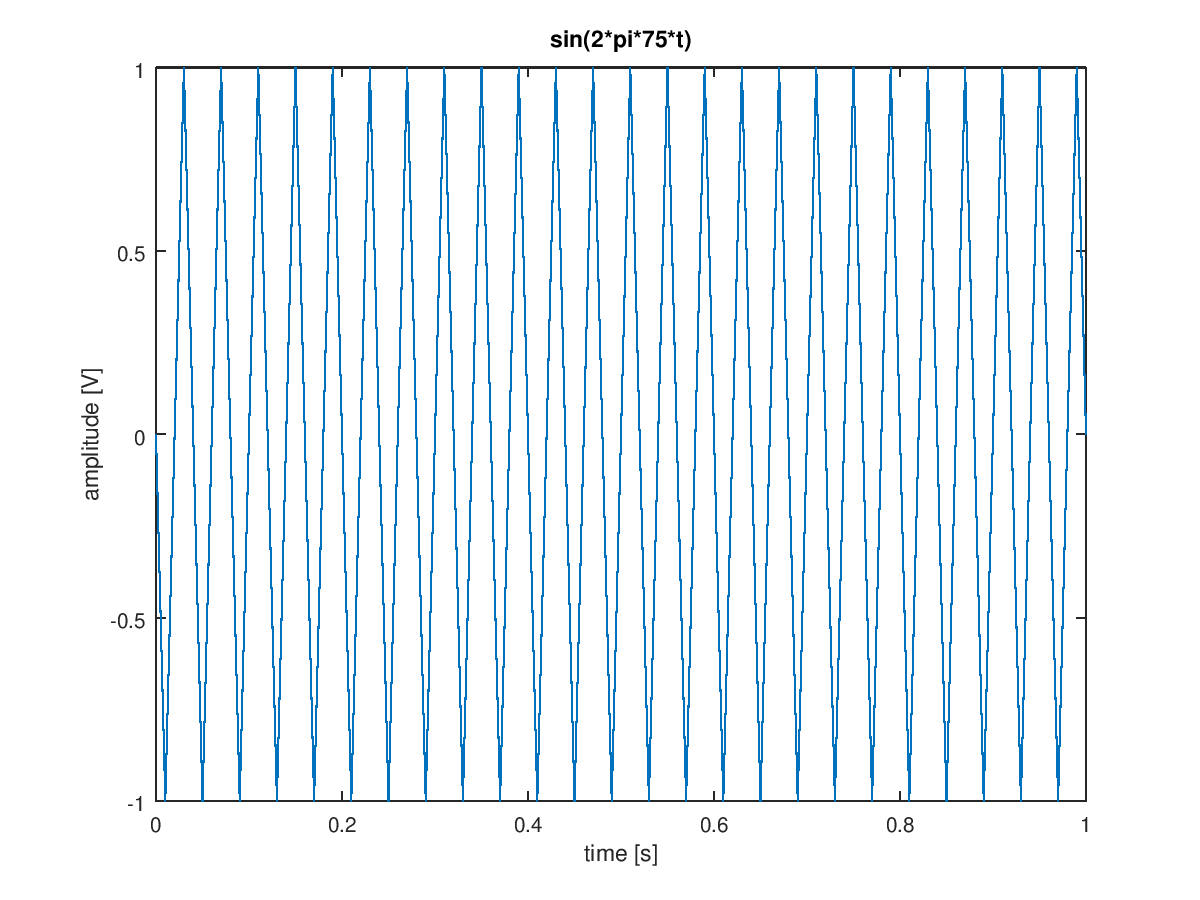
\includegraphics[width=\textwidth]{img/1_16.png}
				\caption{$x(n, 75)$}
				\label{fig:16}
			\end{figure}

			\begin{figure}[H]
				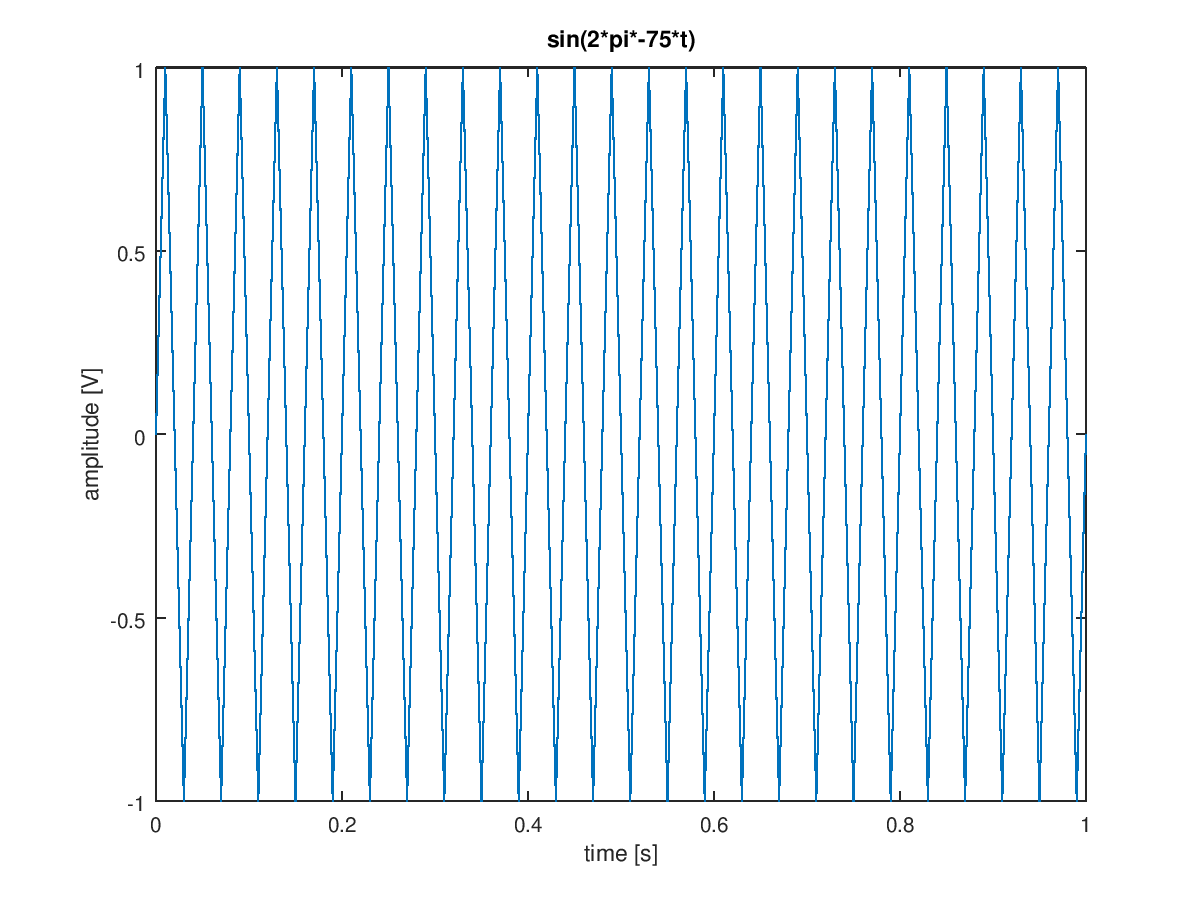
\includegraphics[width=\textwidth]{img/1_17.png}
				\caption{$x(n, -75)$}
				\label{fig:17}
			\end{figure}
		% section sampling_and_aliasing (end)

		\section{Sampling of Signals Which Are Expressible as a Superposition of Trigonometric Functions} % (fold)
		\label{sec:sampling_superposition_of_trigonometric_functions}
			In this section, we inspect what happens to signals when they're composed of more than one frequency. We first consider a signal $s$, where
			\[
				s = \sin(2\pi f_1t) + 2\cos(2\pi f_2 t)
			\]

			Once again we consider a sampling frequency of $f_s = 100 Hz$, and by using the same process as in the previous section, the digitally sampled formula of this message can be expressed as
			\[
				s(n, f_1, f_2) = \sin\left(\frac{\pi}{50} f_1 n\right) + 2\cos\left(\frac{\pi}{50} f_2 n\right), \quad n \in \mathbb{Z}
			\]

			Letting $f_1=10 \text{ Hz},\, f_2 = 30 \text{ Hz}$, we can sketch the spectra of $s(n, 10, 30)$, as shown in \ref{fig:18}. As can be clearly seen, the frequency content is what we expect, as we have frequency components at 10 Hz and 30 Hz, as well as -10 Hz and -30 Hz due to. In theory, however, if we should choose one of our frequency components to be above the Nyquist frequency $f_s/2 = 50$ Hz, then that part of the signal should be aliased. By changing the second frequency component to $f_2 = 60$ Hz, we get the resulting figure \ref{fig:19}. Notice that our second frequency component does not appear as 60 Hz, but rather as 40 Hz, which is obviously not correct. It seems that the aliasing frequencies seem to ``reflect'' around the Nyquist frequency, as $f_2$ is 10 Hz more than the Nyquist frequency of 50 Hz, but the resulting frequency component $f_2'$ is 10 Hz less than the sampling frequency.

			\begin{figure}[H]
				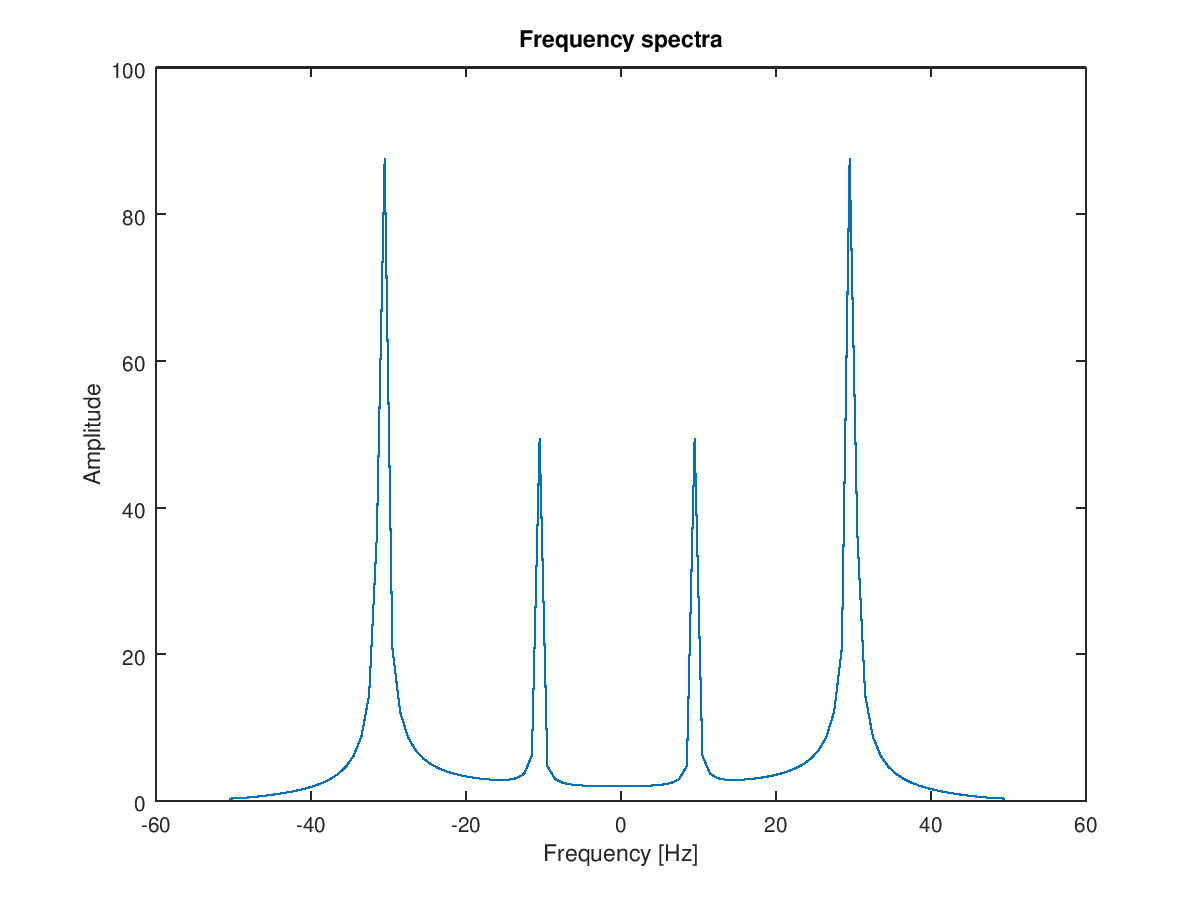
\includegraphics[width=\textwidth]{img/1_18.png}
				\caption{FFT of $s(n, 10, 30)$}
				\label{fig:18}
			\end{figure}

			\begin{figure}[H]
				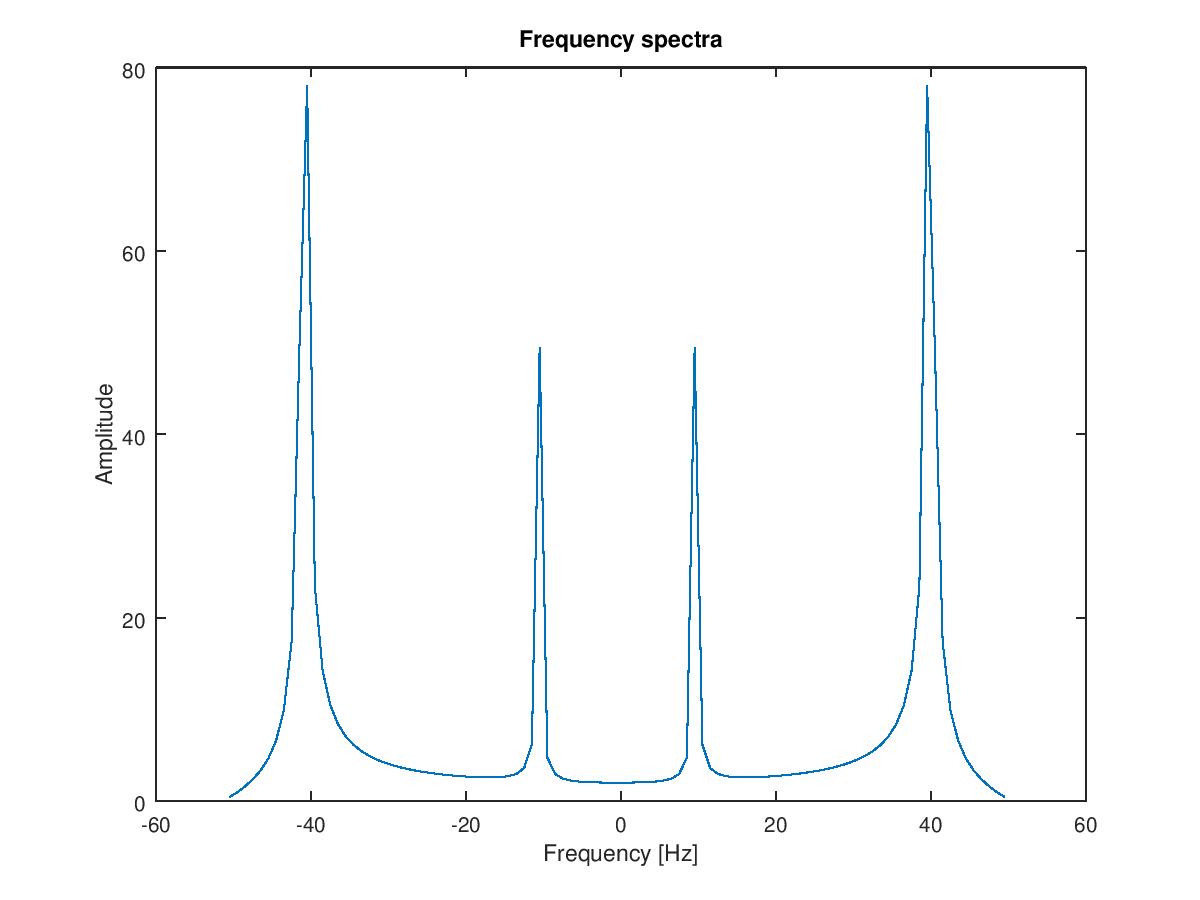
\includegraphics[width=\textwidth]{img/1_19.png}
				\caption{FFT of $s(n, 10, 60)$}
				\label{fig:19}
			\end{figure}
		% section sampling_superposition_of_trigonometric_functions (end)
	% chapter discrete_time_signals_and_systems (end)

	\chapter{Discrete Fourier Transform and Fast Fourier Transform} % (fold)
	\label{cha:discrete_fourier_transform_and_fast_fourier_transform}
		We begin this section by writing code for a Discrete Fourier Transform, the code of which can be found in the appendix. First, we test the code with sample input signals,
		\[
			\begin{array}{rcl}
				x_1 & = & \{1, 1\} \\
				x_2 & = & \{1, 0, 1, -1\}
			\end{array}
		\]

		\noindent Using the \texttt{DFTdir} function, the results are
		\[
			\begin{array}{rcl}
				X_1 & = & \{2, -j\} \\
				X_2 & = & \{1,-j,3,j\}
			\end{array}
		\]

		These results were confirmed to be correct by using a scientific calculator on the Internet.
		\section{Direct DFT vs. FFT} % (fold)
		\label{sec:direct_dft_vs_fft}
			In this section, we compare the direct DFT method and the Fast Fourier Transform. We start by generating 1024 samples of $\sin(2\pi t)$, with the bounds of $t$ between 0 and 2. In a discrete sampling sense, this input can be given as
			\begin{equation}
				\sin\left(2\pi \cdot \frac{2n}{1024}\right) = \sin\left(\frac{\pi n}{256}\right),\quad 0 \le n \le 1024, k\in \mathbb{Z}
				\label{eq:2_sin}
			\end{equation}

			In figure \ref{fig:2_dft}, we show the values of the \texttt{DFTdir} method on the input given in \eqref{eq:2_sin}. The values were simply plotted as indices of the Fourier Transform, as we do not need to shift the output and correct the scaling for frequency in order to draw a comparison. In figure \ref{fig:2_fft}, we see the results of using Octave's built-in \texttt{fft} function with the same input. As can easily be seen, the two functions provide the same output.

			\begin{figure}[H]
				\centering
				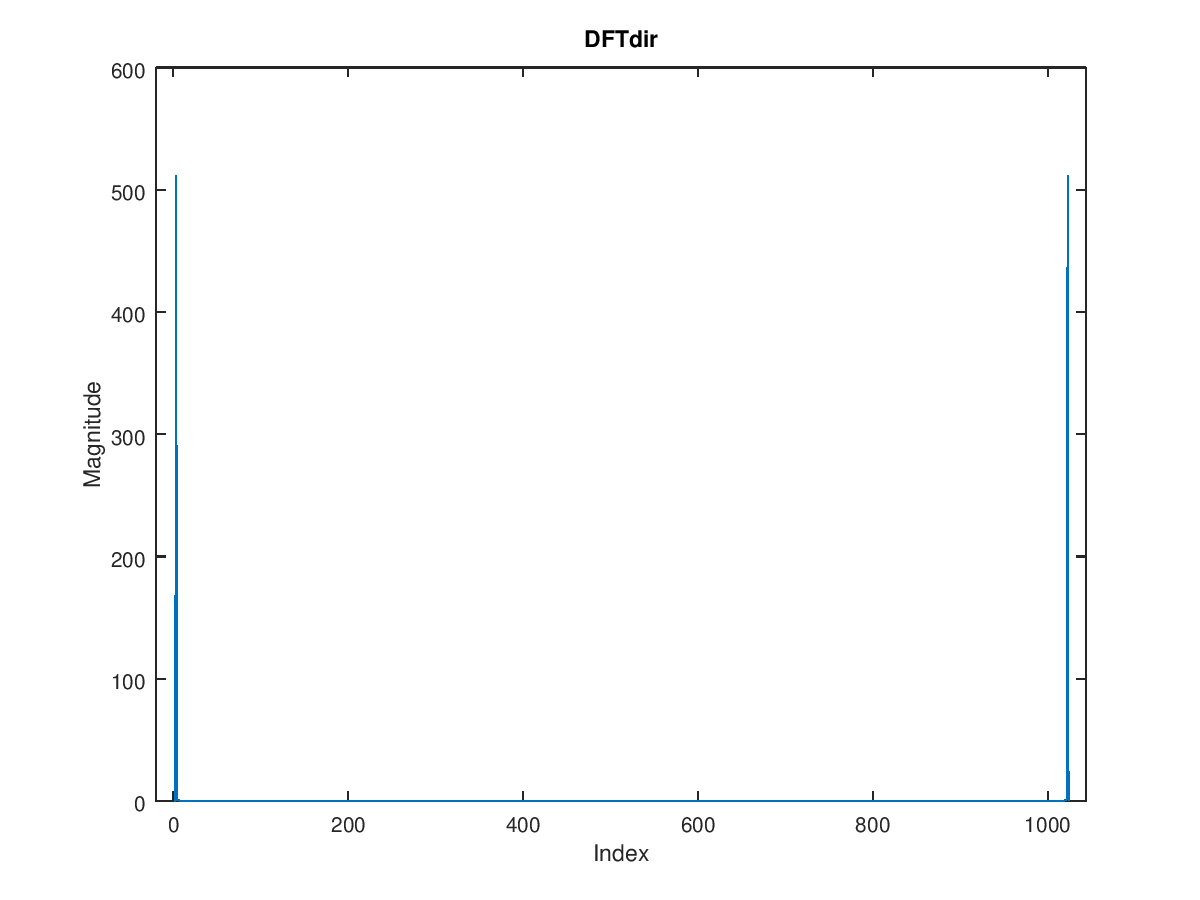
\includegraphics[width=.7\textwidth]{img/2_1.png}
				\caption{\texttt{DFTdir} results for \eqref{eq:2_sin}}
				\label{fig:2_dft}
			\end{figure}

			\begin{figure}[H]
				\centering
				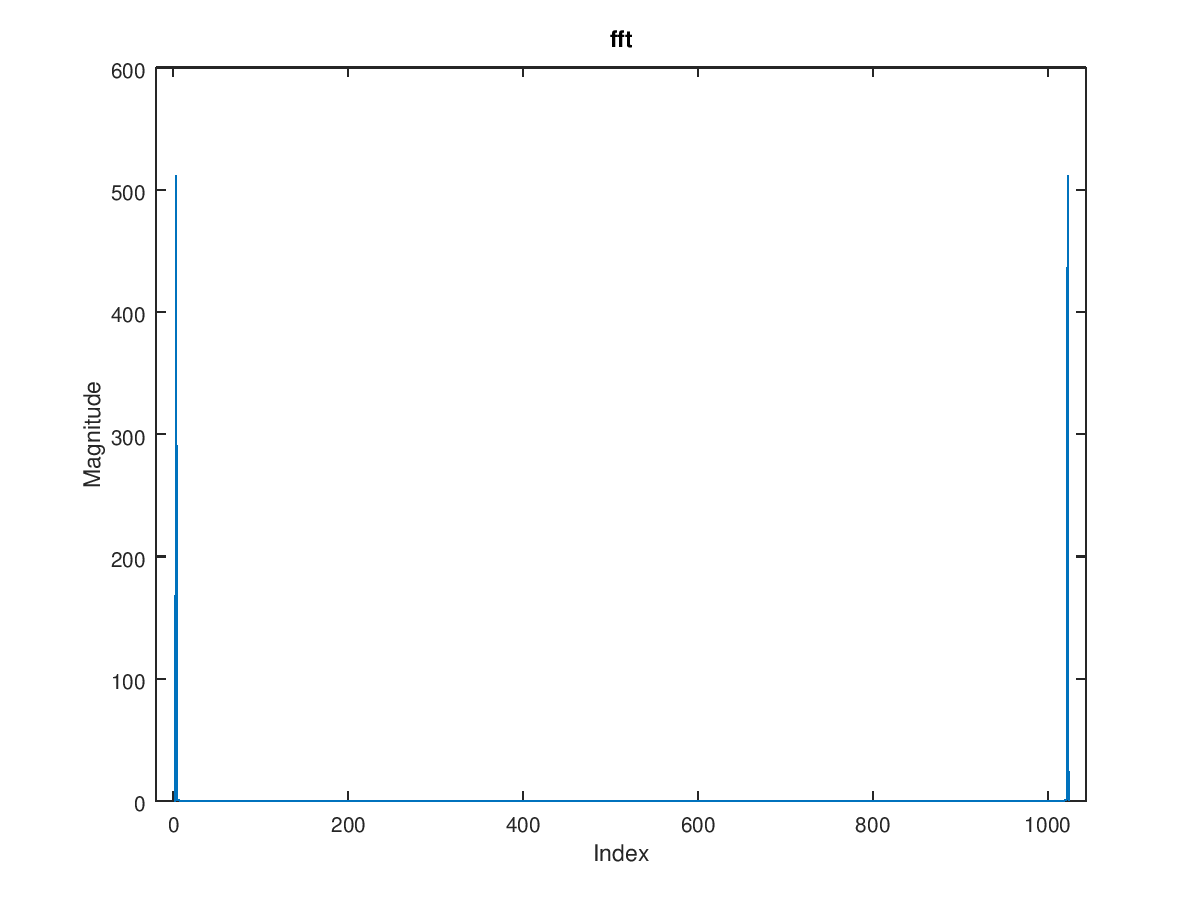
\includegraphics[width=.7\textwidth]{img/2_2.png}
				\caption{Octave's \texttt{fft} results for \eqref{eq:2_sin}}
				\label{fig:2_fft}
			\end{figure}

			At this point, we perform a performance comparison of the two methods. By modifying the \texttt{DFTdir} method as in \textit{add new code to appendix}, we compute the average time taken to compute 20 runs of the \texttt{DFT\_dir} of \eqref{eq:2_sin}, and see that the time it takes to compute the output in figure \ref{fig:2_dft} is approximately 9.64 seconds, with a standard deviation of $\rho_{DFT} = 0.21$ seconds. Performing the function given by \textit{add code to appendix} the time is drastically reduced to $87.92 \,\mu$s, with a standard deviation of $\rho_{fft} = 28.19 \,\mu s$. The results for individual runs of the functions can be seen in figures \ref{fig:2_dft_performance} and \ref{fig:2_fft_performance}.

			\begin{figure}[H]
				\centering
				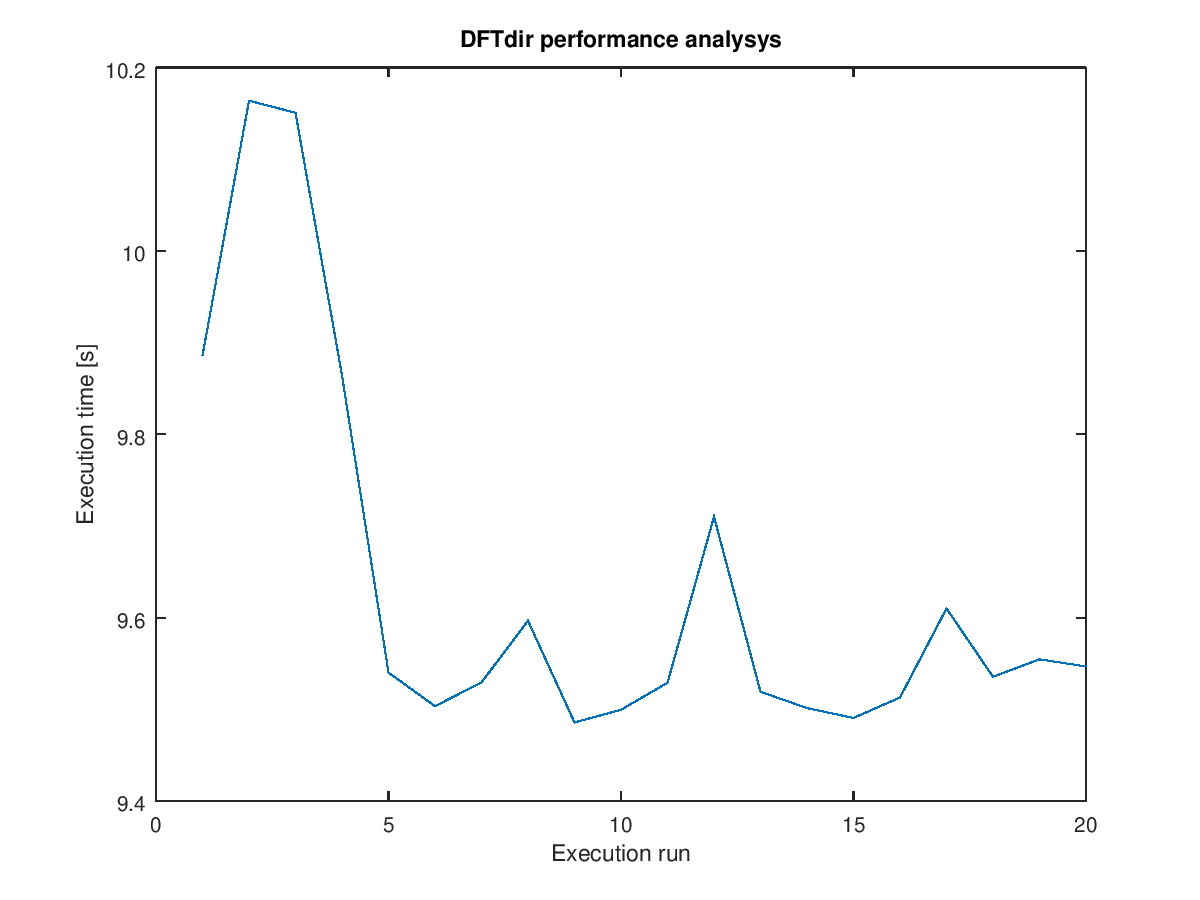
\includegraphics[width=.8\textwidth]{img/2_3.png}
				\caption{\texttt{DFTdir} algorithm runtimes with \eqref{eq:2_sin} as input}
				\label{fig:2_dft_performance}
			\end{figure}

			\begin{figure}[H]
				\centering
				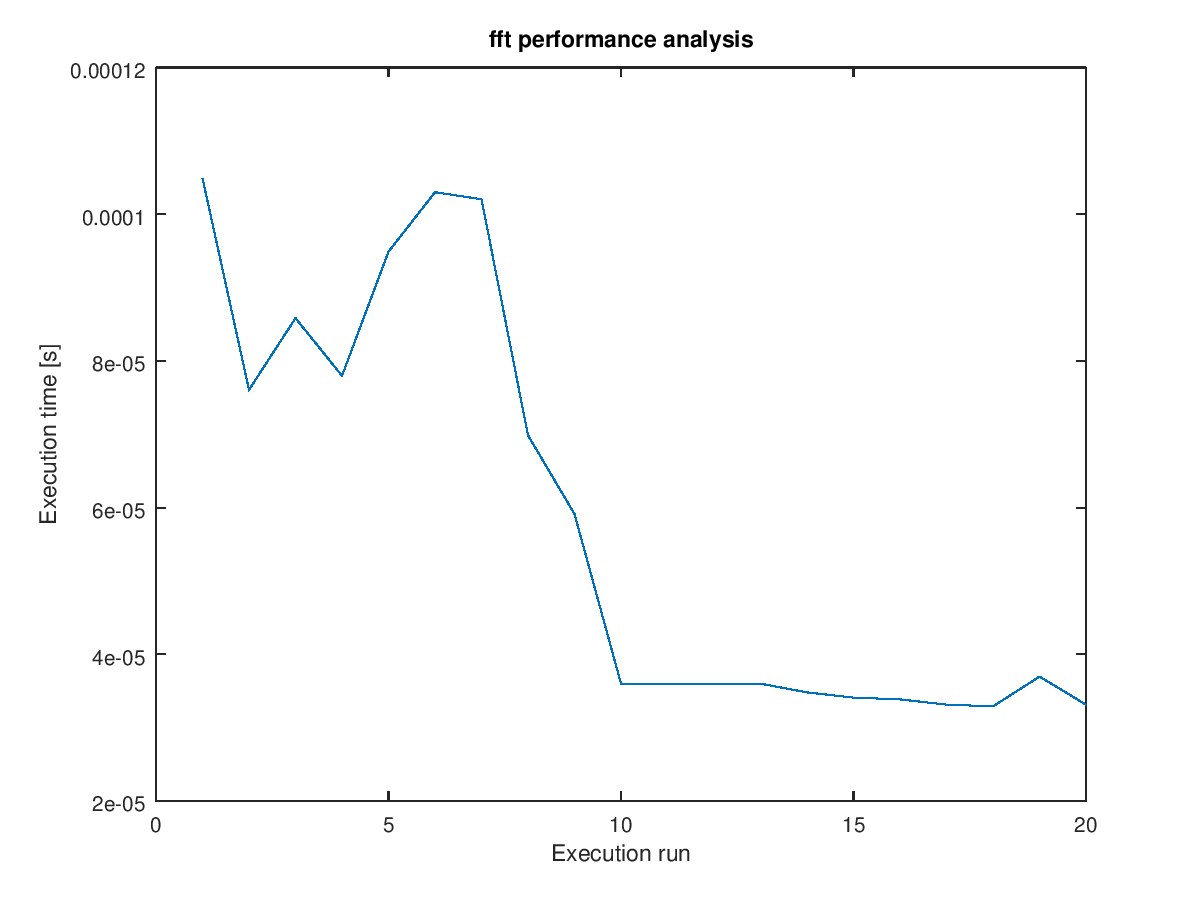
\includegraphics[width=.8\textwidth]{img/2_4.png}
				\caption{\texttt{fft} algorithm runtimes with \eqref{eq:2_sin} as input}
				\label{fig:2_fft_performance}
			\end{figure}

			The following table are results for values of \eqref{eq:2_sin} for larger values of $N$, the number of samples given to be computer
			\begin{table}[H]
				\begin{tabularx}{\textwidth}{X X X X X}
					\toprule
					& \multicolumn{2}{c}{\texttt{DFTdir}} & \multicolumn{2}{c}{\texttt{fft}} \\
					$N$ & Average (s) & $\rho_{DFT}$ & Average (s) & $\rho_{fft}$ \\
					\midrule
					2048 & 38.51 & 0.107 & $3.65 \times 10^{-4}$ & $1.43 \times 10^{-3}$ \\
					4096 & 152.6 & 0.38 & $2.75 \times 10^{-4}$ & $1.05 \times 10^{-3}$ \\
					8192 & - & - & $3.7 \times 10^{-4}$ & $1.44 \times 10^{-3}$ \\
					\bottomrule
				\end{tabularx}
				\caption{Results for different values of $N$ for each algorithm}
			\end{table}
		% section direct_dft_vs_fft (end)
	% chapter discrete_fourier_transform_and_fast_fourier_transform (end)

	\appendix
	\chapter{DFTdir code} % (fold)
	\label{sec:dftdir_code}
		\texttt{function out = DFTdir (input);}\par
		\texttt{out = zeros(1, length(input));}\par
		\indent\texttt{N = length(input);}\par
		\texttt{for k = 0:N-1}\par
		\hspace*{2em}\texttt{temp = 0;}\par
		\hspace*{2em}\texttt{for n = 0:N-1}\par
		\hspace*{4em}\texttt{temp += input(n + 1) * exp(-i*2*pi*k*n/N);}\par
		\hspace*{2em}\texttt{endfor}\par
		\hspace*{2em}\texttt{out(k + 1) = temp;}\par
		\texttt{endfor}\par
		\noindent\texttt{endfunction}\par
	% section dftdir_code (end)
\end{document}